% !TEX root = ../main.tex
\fancychapter{Introduction}%
\label{chap:intro}
\cleardoublepage{}

\noindent
Modern \ac{CAD} applications include substantial support for parametric
operations and \ac{GCS}.  These mechanisms have been developed over the past few
decades~\cite{Bettig:2011:GCSPC} and are heavily and ubiquitously used across
the \ac{AEC} industry.

Parametric modeling is used to design with constraints, whereby users express a
set of parameters and interdependent operations, establishing restrictions
between geometric entities.  The resulting geometry can be controlled from input
parameters using two computational mechanisms:
\begin{enumerate*}[label= (\arabic*)]
  \item parametric operations, which build geometry that implicitly abides by
  constraints imposed when the user selects the operation and its inputs, and
  \item \ac{GCS}, which manipulates geometry in sketches and models to satisfy
  constraints explicitly imposed on objects by the user.
\end{enumerate*}

Nowadays, Parametric operations in \ac{CAD} software are mostly accessible
through intuitive, robust, and easy to use direct-manipulation interfaces,
offering a wide variety of different operations.  These operations are created
when a designer uses solid modeling operations, such as face extrusions or shape
unions; and recorded into a user-controlled sequential history of construction
steps that can be replayed in the face of changes, updating the modeled
geometry.  Alas, dependency propagation direction is fixed, forcing users to
plan their model's features beforehand.  Contrastingly, in constraint solving,
dependency propagation direction isn't fixed.  Instead, users introduce a set of
parameters and geometric entities followed by specifying the constraints that
relate these objects.  Naturally, \ac{GCS} fits in \ac{CAD} software, having
been target of considerable research and development to implement efficient
approaches and methodologies capable of solving \ac{GC} problems.  So much so
that it has become standard in major \ac{CAD} software, such as
AutoCAD~\cite{Autodesk:1982:AutoCAD}, which supports the ability to constrain
objects in a variety of ways, e.g., point coincidence, line perpendicularity,
tangencies, among other kinds of constraints.

However, traditional interactive methods for parametric modeling suffer from the
disadvantage that they do not scale properly when designing more complex ideas.
In recent years, a novel approach to design named \ac{AD} has emerged,
introducing the algorithmic methodology also present in the \ac{CS} field,
allowing the specification of sketches and models through
algorithms~\cite{McCormack:2004:GDPDR}, leading to the creation and integration
of several \ac{AD} tools into \ac{CAD} software as well.  Some use \acp{VPL},
others \acp{TPL}, or even a mixture of both.  The latter overcomes a fundamental
issue with \acp{VPL} which is the frequently disproportionate complexity between
the program and the respective resulting model.

\acp{TPL} come with some advantages over \acp{VPL}, among which are
\begin{enumerate*}[label= (\arabic*)]
  \item abstraction mechanisms, enabling the encapsulation of behavior that can
  be changed and reused in a different context at a later time,
  \item the ability of specifying recursive definitions,
  \item resulting source code can be put under a version control system, and
  \item multiple developers can work on the same codebase.
\end{enumerate*}
In spite of these, dealing with \acp{GC} remains a arduous task.  Take as an
example the sketch of a chair seat's outer frame, as seen in
\cref{fig:intro.chair}, from a multi-purpose chair generation
tool~\cite{Garcia:2012:ChairDNA} where the chair's overall shape is controllable
by specifying the values for a set of input parameters.

\begin{figure}[htbp]
  \centering
  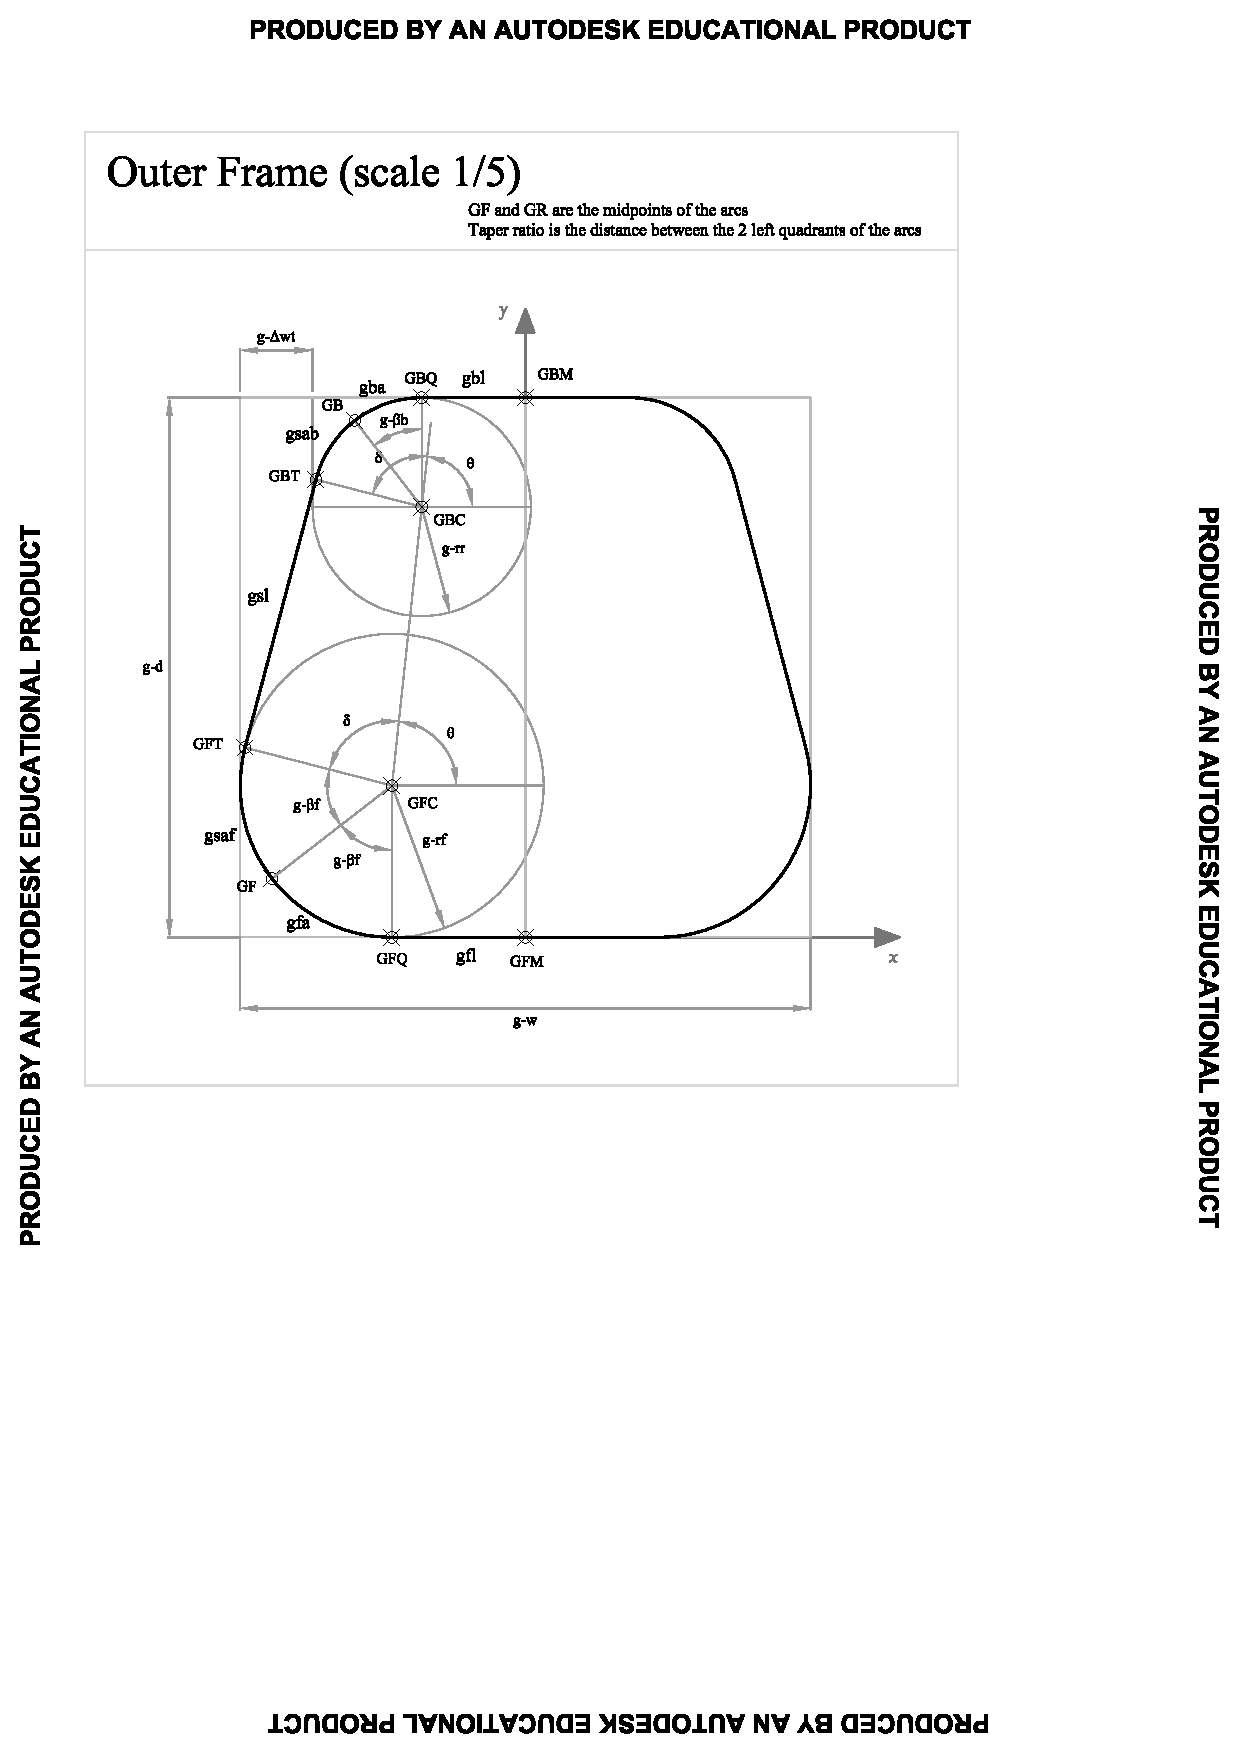
\includegraphics[width=.6\textwidth]{fig/chair-seat-outer-frame}\par
  {\scriptsize Source: Project source code, publicly unavailable (Jan 2019)}
  \caption[Sketch of a chair seat's outer frame]{
    Sketch of a chair seat's outer frame, defined by 5 input parameters:
    \begin{enumerate*}[label= (\arabic*)]
      \item Width ($g-w$),
      \item depth ($g-d$),
      \item taper width ($g-\Delta wt$),
      \item front radius ($g-rf$), and
      \item rear radius ($g-rr$).
    \end{enumerate*}}%
  \label{fig:intro.chair}
\end{figure}

The seat's corners are defined by circles whose respective front and rear
radius' length, $g-rf,g-rr$, is obtained by computing distances, from which the
circles' centers, $GFC$ and $GBC$, can be obtained.  The circles are then
connected through outer tangent lines, $gsl$, forming the outer frame of the
chair's seat.  Some of these operations, such as the radius computation,
\textit{tangency}, and \textit{circumcenter}, depend on operations that query if
a point is at a certain distance from an object, or if two points are
coincident.  Such operations must be handled carefully due to numerical
robustness issues that may arise when performing fixed-precision arithmetic.  As
such, on top of the design process itself, the user must identify these kinds of
\acp{GC}, resorting to trigonometry analysis, perform tolerance-based
comparisons to determine point distance or if two points are coincident, among
other techniques the user most likely is not aware he must rely upon to
circumvent these issues, particularly, when we take into consideration that most
designers using \ac{AD} are architects and designers without an extensive
background in \ac{CS}.

To overcome the limitations exposed above, this report proposes the
implementation of a wide variety of \ac{GC} primitives with
specialized efficient solutions for different combinations of input objects.  In
this manner, the user won't have to be aware of numerical robustness issues and
have to investigate techniques for solving such issues to accurately generate a
model riddled with \acp{GC}.

\section{Document Structure}%
\label{sec:intro.structure}

The present document is structured in \total{chapter} different chapters,
namely:
\begin{description}
  \item[\nameref{chap:intro}] Broken into several sections, including this
  one, presents:
  \begin{enumerate*}[label= (\arabic*)]
    \item A brief historical overview of the development of parametric
    operations in \ac{CAD} software in \cref{sec:intro.parametric},
    \item the main approaches to \ac{GCS} in \ac{CAD}, in
    \cref{sec:intro.constraints},
    \item two simple algebraically formulated examples of \ac{GC} problems and
    respective solutions along with code examples, in \cref{sec:intro.examples},
    and
    \item a section dedicated to further elaborating on \ac{AD} and the benefits
    and drawbacks it introduces to the design process, in \cref{sec:intro.ad}.
  \end{enumerate*}

  \item[\nameref{chap:related}] An exposition of the related work in the form of
  \begin{enumerate*}[label= (\arabic*)]
    \item a comprehensive discussion about numerical robustness in computational
    processes, showcasing a set of software tools capable of handling these
    issues in the context of geometric computation, in
    \cref{sec:related.robustness},
    \item an overview of some \ac{GC} tools, presenting some of their benefits
    and drawbacks, in \cref{sec:related.constraints}, and
    \item an overview of algorithmic design tools, similarly comparing them and
    addressing positive and negative points, in \cref{sec:related.ad}.
  \end{enumerate*}

  \item[\nameref{chap:solution}] A detailed solution proposal, including an
  explanation of how its implementation can be capable of efficiently handling
  the specification of \ac{GC} problems, in \cref{chap:solution}.

  \item[\nameref{chap:evaluation}] A brief plan of the methodology used to evaluate
  the proposed solution in \cref{chap:evaluation}.

  \item[\nameref{chap:conclusion}] Concluding remarks that summarize the
  document, in \cref{chap:conclusion}.
\end{description}

% !TEX root = ../../main.tex
\section{Parametric Operations in \acs{CAD}}
\label{sec:intro.parametric}

Despite never using the word \textit{parametric} in writing, Ivan Sutherland
introduced the world to Sketchpad \cite{Sutherland:1964:Sketchpad} in 1963, an
interactive 2D \ac{CAD} program capable of establishing atomic constraints
between objects which had all the essential properties of a parametric equation,
being the first of its kind and the prime ancestor of modern \ac{CAD} programs.
The earliest 3D parametric system \cite{Requicha:1980:RRS:356827.356833} dates
from the 1970s.  It used a \ac{CSG} \cite{Foley:1996:CGPP,Requicha:1977:CSG}
binary tree, and \ac{B-Rep} \cite{Stroud:2006:BRMT} for representing solid
objects.  This system's parametric nature rested in the \ac{CSG} tree, which
acted as a rudimentary construction step history.  The user could make
modifications to the controlling parameters' values of a certain operation in
the tree, reapply the modified history, and generate the newly updated model.
Nearly a decade later, the first parametric system as it is understood today
\cite{Jabi:2013:PDA,PTC:1980:ProENGINEER} surfaced, enabling the establishment
of relations between the objects' sizes and positions such that a change in a
dimension between objects would automatically move or change affected objects
accordingly.  Unlike Sketchpad, it supported 3D geometry and changes would
propagate over different drawings made by different users.  This lead to the
appearance of dimensions and \acp{GC} in parametric operations, having \ac{GCS}
in drawings become standard by the early 1990s
\cite{Bouma:1995:GCS,Chung:1990:TEVPD,Owen:1991:ASGDC}.  Efforts to expand the
benefits of constraint solving beyond simple sketches were made, having the
majority of some systems implemented constraint solving in 3D.  Improvements
from then on focused mostly on robustness and operation variety.

In recent decades, emphasis shifted to making parametric \ac{CAD} software more
interactive and user friendly.  The intent was to make it as simple as dragging
a face of an object to where it should be instead of scrolling through a
construction history in attempts to locate a specific operation, and hopefully
changing the correct controlling parameter's value within that operation.  This
in itself is a tedious and error-prone process that can lead to undesired
side-effects instead of producing the intended changes.  A variety of systems
have been developed to mitigate this rigidity
\cite{Clarke:2009:SM,Samuel:2006:CPPUP,Wu:2007:MSMSM}, but not without
drawbacks, since direct-manipulation operations were just added to the
construction history as transformation operations, oblivious to parent
operations the new ones might depend on.  Further limitations are discussed in
\cite{Bettig:2005:LPOSSD}, along with a proposal for future design software
exempt of parametric operations.  Nonetheless, parametric operations will still
see continued usage for the foreseeable future.

% !TEX root = ../../main.tex
\section{Constraints in \acs{CAD}}%
\label{sec:intro.constraints}

We've seen how parametric operations in \ac{CAD} software have evolved.  These
operations allow the user to create geometric objects that satisfy certain
constraints \textit{implicitly} imposed on the objects when the user selects the
operations they want to use along with the respective operation's inputs.
Naturally, \ac{GCS} fits well in \ac{CAD} applications.  \Acp{GC} allow the
repositioning and scaling of geometric objects so that they satisfy constraints
\textit{explicitly} imposed on them by the user.

\acp{CSP} are a well-known subject of research both in mathematics and in the
\ac{CS} field.  \ac{GCS} is a subclass of \acp{CSP}. More specifically, it is a
\ac{CSP} in a computational geometry setting.  The abstract problem of \ac{GCS}
is often described as follows~\cite{Bettig:2011:GCSPC}:

\begin{quote}
  Given a set of geometric objects, such as points, lines, and circles; a set of
  geometric and dimensional constraints, such as distance, tangency, and
  perpendicularity; and an ambient space, usually the Euclidean plane; assign
  coordinates to the geometric objects such that the constraints are satisfied,
  or report that no such assignment has been found.
\end{quote}

One of the important features of a solver is its \textit{competence}, which is
related to the capability of reporting unsolvability: if in fact no solution for
the problem at hand exists and the solver is capable of reporting unsolvability
in that case, the solver is deemed fully competent.  Since constraint solving is
mostly an exponentially complex problem~\cite{Rossi:2006:Handbook}, partial
competence suffices as long as decent solutions can be found in affordable time
and space.

There are multiple approaches to constraint solving, but the most relevant ones
are graph-based, logic-based, algebraic, and theorem prover-based, of which the
first is the predominant one.  It is important for these approaches that the
\ac{GC} system does not have too few or too many constraints.  Summarily, a
system can either be 
\begin{enumerate*}[label= (\arabic*)]
  \item under-constrained if the number of solutions is unbound due to lack of
  constraint coverage over the entities involved,
  \item over-constrained if there are no solutions because of constraint
  contradictions, or
  \item well-constrained if the number of solutions is bound to a finite
  positive number.
\end{enumerate*}

Some of the subjects approached here are briefed in~\cite{Hoffmann:2005:BCS}.
The following sections present and briefly discuss the aforementioned approaches
to constraint solving.

\subsection{Graph-Based Approaches}%
\label{sec:intro.constraints.graph}

In graph-based approaches, the problem is translated into a labeled
\textit{constraint graph}, where vertices are constrained geometric objects, and
edges the constraints themselves.  This approach is split into three main
branches:

\begin{itemize}
  \item[] \textbf{Constructive Approaches} The graph is decomposed and
  recombined to extract basic construction steps that must be solved, where a
  subsequent phase elaborates on this, employing algebraic and/or numerical
  methods.  This has become the dominant approach to \ac{GCS}, also becoming the
  target of considerable research and
  development~\cite{Bettig:2011:GCSPC}.

  \item[] \textbf{Degrees of Freedom Analysis} The graph's vertices are labeled
  with represented object's degrees of freedom.  Each edge is labeled by the
  degrees of freedom the constraint cancels out.  This graph is then analyzed
  for a solution strategy.

  A symbolic solution method is derived using rules with geometric meaning, a
  method proved to be correct in~\cite{Kramer:1990:SGCS}.  It is further
  extended by using it along with numerical methods as a fallback if geometric
  reasoning fails~\cite{Hsu:1997:HCSEIGC}.

  \Citet{Latham:1996:CA} decompose the graph into minimal connected components
  they call \textit{balanced sets} that are solved by a geometric construction,
  falling back to a numerical solution attempt.  This method can deal with
  symbolic constraints and identifies under- and overconstrained problems, where
  the latter kind is approached by prioritizing the given constraints.

  \item[] \textbf{Propagation Approaches} The graph's vertices represent
  variables and equations, and the edges are labeled with occurrences of the
  variables in equations.  The goal is to orient the graph such that all
  incident edges to an equation vertex but one are incoming edges.  If so, the
  equation system has been triangularized.  Orientation algorithms include
  degree-of-freedom propagation and propagation of known
  values~\cite{Freeman:1990:ICS,Veltkamp:1992:Geometric} which can fail in the
  presence of orientation loops, but such situations are
  addressed~\cite{Veltkamp:1992:Geometric} and they may resort to numerical
  solvers.
\end{itemize}

\subsection{Logic-Based Approaches}%
\label{sec:intro.constraints.logic}

Using logic-based approaches, the constraint problem is translated into a set of
geometric assertions and axioms which is then transformed in such a way that
specific solution steps are made explicit by applying geometric reasoning.  The
solver then takes a set of construction steps and assigns coordinate values to
the geometric entities.

A geometric locus\footnote{In mathematics, a locus is a set of points that
satisfy some condition.  In layman's terms, a location or place.} at which
constrained elements must be is obtained using first order logic to derive
geometric information, applying a set of axioms from Hilbert's
geometry~\cite{Aldefeld:1988:VGBGRM,Sohrt:1991:IC3DM,Bruderlin:1993:USGRRSGSS}.
Two different types of constraints are further
considered~\cite{Sunde:1987:CADSDSS,Verroust:1992:RMPCAD}:
\begin{enumerate*}[label= (\arabic*)]
  \item sets of points placed with respect to a local coordinate frame, and
  \item sets of straight line segments whose directions are fixed.
\end{enumerate*}
The reasoning is performed by applying a rewriting system on the sets of
constraints.  Once every geometric element is in a unique set, the problem is
solved.

\subsection{Algebraic Approaches}%
\label{sec:intro.constraints.algebraic}

In the case of an algebraic approach, the problem is translated into a system of
equations where the variables are coordinates of geometric elements and the
equations, which are generally nonlinear, express the constraints upon them.
This approach's main advantage is its completeness and dimension independence.
However, it is difficult to decompose the equation system into subproblems, and
a general, complete solution of algebraic equations is inefficient.
Nonetheless, small algebraic systems tend to appear in the other approaches and
are routinely solved.

\subsection{Symbolic Methods}%
\label{sec:intro.constraints.symbolic}

Symbolic methods rely on general equation solvers which employ symbolic
techniques to triangularize equation
systems~\cite{Chou:1988:IWMMTPG,Buchberger:1995:Grobner} that emerge from
emplying an algebraic approach.  A solver built on top of the Buchberger's
algorithm is described in~\cite{Buchanan:1993:CDS}; \Citet{Kondo:1992:AMMDRGM}
further reports on a symbolic algebraic method.

These methods are powerful since they can produce generic solutions if
constraints are used symbolically, which can be evaluated for a different set of
constraint assignments, then producing parameterized solutions.  However,
solvers are very slow and computations demand a lot of space, usually requiring
exponential running time~\cite{Durand:1998:SNTCS}.

\subsection{Numerical Methods}%
\label{sec:intro.constraints.numerical}

Among the oldest approaches to constraint solving, numerical methods solve large
systems of equations iteratively.  Methods like Newton iteration work properly
if a good approximation of the intended solution can be supplied and the system
is not ill-conditioned.  Take, for example, a sketch of a model the user drew.
If the starting point comes from said sketch, then it should follow that the
result be close to what is intended.  Alas, such methods may find only one
solution, even in cases where there are many, and may not allow the user to
select the one they are interested in.  Such methods are called local methods,
as opposed to global methods, exploring the problem space for every possible
solution.

Relaxation
methods~\cite{Sutherland:1964:Sketchpad,Hillyard:1978:CNSTDT,Borning:1989:PLATL}
can be employed in attempts to partly minimize global error by perturbing the
values assigned to the variables.  However, in general, convergence to a
solution is slow.

The Newton-Raphson iteration method, the most widely used one, is a local method
and converges much faster than relaxation, but does not apply to
over-constrained systems of equations unless expanded
upon~\cite{Dedieu:2000:Newton}.

Global and guaranteed convergence can be had resorting to the \textit{Homotopy
continuation} family of methods~\cite{Allgower:1993:CPF}.  Despite usage in
\ac{GCS}~\cite{Lamure:1996:SGCH,Durand:1998:SNTCS}, these are far less efficient
than the Newton-Raphson method due to the latter's exhaustive nature.

\subsection{Theorem Proving}%
\label{sec:intro.constraints.proving}

\ac{GCS} can be seen as a subproblem of geometric theorem proving, but the
latter requires general techniques, therefore requiring much more complex
methods than those required by the former.

Wen-Tsün Wu's Wu-Ritt method~\cite{Wu:1984:BPMCTPG,Wu:1994:MTPG} is an
algebraic-based method that can be used to automatically find necessary
conditions to obtain non-degenerated solutions.  It can be used to prove novel
geometric theorems~\cite{Chou:1988:IWMMTPG}.
\Citet{Chou:1996:AGRPGI:1,Chou:1996:AGRPGI:2} develop on automatic geometric
theorem proving, allowing the interpretation of the computed proof.

\subsection{Other Areas}%
\label{sec:intro.constraints.other}

The following are briefly described key advances made during the past two
decades that interface with other areas or that cannot be readily integrated
into graph-constructive solvers.  These techniques also constitute examples of
further attempts to broaden the scope of \ac{GCS}, proving that it is a strong
field of research with many applications beyond \ac{CAD}.

\begin{itemize}
  \item[] \textbf{Deformations} When restrictions are placed on the type of
  deformation, these problems can be seen as constraint solving.  For
  example, \citet{Ahn:2014:GCQBCUML,Bao:2010:BIVCMSE,Moll:2006:PPDLO} consider
  deformations that minimize strain energy; \Citet{Xu:2009:SDUAC} entail
  surface deformation under area constraints.  However, such techniques are
  rarely integrated with other \acp{GC} such as point distance or
  perpendicularity.
  \item[] \textbf{Dynamic Geometry} The addition of constraints to a given
  under-constrained system can make it well-constrained, and such constraints
  can be seen as parameters when they are dimensional.  Varying their values,
  different solutions arise, which can be wholly understood as a dynamic
  geometric configuration.  Systems akin to
  Cinderella~\cite{Richter:2012:Cinderella.2} can deal with these problems.
  Further literature exists on these problems from a constraint solving
  perspective~\cite{Freixas:2010:CDGS}.
  \item[] \textbf{Evolutionary Methods} Consist of re-interpreting the problem
  as an optimization problem, attacking it using genetic, particle-swarm or
  other evolutionary methods~\cite{Chunhong:2006:PDBOEA,Li:2012:HASPSOASGCP}.
\end{itemize}

% !TEX root = ../../main.tex
\section{\acl{GC} Problem Examples}%
\label{sec:intro.examples}

This section presents two simple examples of geometric models that are defined
through the specification of \acp{GC}, and the respective solutions using
intuitive algebraic formulation, accompanied by programmatic solutions.
Depictions of the aforementioned models can be seen in \Cref{fig:intro.example}.
The examples are limited to the two-dimensional Euclidean plane over real
numbers, $\mathbb{R}^2$.  Solutions for analogous problems in three-dimensional
Euclidean space, $\mathbb{R}^3$, exist as well.

\begin{figure}[htpb]
  \centering
  \subcaptionbox{\label{fig:intro.example.parallel}%
    Line that goes through $C$, strictly parallel to $\overleftrightarrow{AB}$}
    [.45\linewidth]{\resizebox{!}{.2\textheight}{\begin{tikzpicture}[rotate=20]
  \tkzDefPoints{0/0/A,3/0/B,1/1/C}
  \tkzDefLine[parallel=through C](A,B) \tkzGetPoint{D}
  \tkzDrawLines[add=.1 and .1](A,B C,D)
  \tkzDrawPoints(A,B,C)
  \tkzLabelPoints(A,B,C)
\end{tikzpicture}
}}
  \subcaptionbox{\label{fig:intro.example.circumcenter}%
    $\odot O_r$ circumscribed about $\triangle ABC$}
    [.45\linewidth]{\resizebox{!}{.2\textheight}{\begin{tikzpicture}
  \tkzDefPoints{0/0/A,1/3/B,4/0/C}
  \tkzCircumCenter(A,B,C) \tkzGetPoint{O}
  \tkzDefMidPoint(A,B) \tkzGetPoint{AB}
  \tkzDefMidPoint(A,C) \tkzGetPoint{AC}
  \tkzDefMidPoint(B,C) \tkzGetPoint{BC}
  \tkzDrawSegments[style=dashed](AB,O AC,O BC,O)
  \tkzMarkRightAngles(A,AB,O B,BC,O C,AC,O)
  \tkzDrawPolygon(A,B,C)
  \tkzDrawCircle(O,A)
  \tkzDrawSegment(O,A)
  \tkzDrawPoints(A,B,C,O)
  \tkzLabelLine[above](O,A){$r$}
  \tkzLabelPoints[below left](A)
  \tkzLabelPoints[above left](B)
  \tkzLabelPoints[below right](C)
  \tkzLabelPoints(O)
\end{tikzpicture}
}}
  \caption[Geometric models defined using GCs]{
    Geometric models defined using \ac{GC} relations:
    \subref{fig:intro.example.parallel} showcases line parallelism, and
    \subref{fig:intro.example.circumcenter} showcases a circle circumscription
    about a triangle.}\label{fig:intro.example}
\end{figure}

The first problem is that of a parallelism constraint: specifying a line that
goes through a given point while also being strictly parallel to another already
defined line.  The second problem is a circumscription constraint: defining a
circle that tightly wraps around a triangle, i.e., the circle's circumference
goes through three given non-collinear points.

\subsection{Parallel lines}%
\label{sec:intro.examples.parallel}

Let $A,\,B,\,C \in \mathbb{R}^2$ such that $C$ is a point in the line which is
strictly parallel to the line $\overleftrightarrow{AB}$ (see
\cref{fig:intro.example.parallel}).

A line in $\mathbb{R}^2$ can be described by the parametric equation
\begin{equation}\label{eq:line.parametric.2}
  P_Q = Q + \lambda\vec{u} \Rightarrow
  \begin{cases}
    x = x_Q + \lambda u_x \\
    y = y_Q + \lambda u_y
  \end{cases}
  ,\,\lambda \in \mathbb{R}
\end{equation}\equations{Parametric equation of a line in $\mathbb{R}^2$}
where $Q = (x_Q, y_Q)$ is a point on the line that goes through $P_Q = (x, y)$,
and $\vec{u} = (u_x, u_y)$ is the vector that drives the line.  To then describe
the line that goes through $C$ and is parallel to $\overleftrightarrow{AB}$, one
must compute the base point $Q$, trivially $C$, and the directional vector
$\vec{u}$, which can be obtained from $\overleftrightarrow{AB}$.  Let $Q = C$,
and $\vec{u} = B - A$, such that, from \cref{eq:line.parametric.2},
\[
  P_C = C + \lambda \vec{u},\,\lambda \in \mathbb{R}.
\]

\Cref{lst:intro.example.parallel.tikz} shows the code used to produce the
example shown in \Cref{fig:intro.example.parallel} using
TikZ~\cite{Tantau:2015:tikz-manual} with the \texttt{tkz-euclide} \LaTeX{}
package, using \texttt{tkzDefLine}, which takes two points $A,\,B$, with the
\texttt{parallel} transformation option.  This option takes the point $C$ the
resulting line goes through.  The result is a point $D = C + \vec{u}$, which can
be obtained using \texttt{tkzGetPoint} to later draw the line. 

\begin{listing}[htb]
  \inputminted[highlightlines=3]{latex}{tikz/ex-parallel.tex}
  \caption[Parallel lines example using \texttt{tkz-euclide}]{
    Parallel lines example from \cref{fig:intro.example.parallel} using
    \texttt{tkz-euclide}.  The highlighted line shows how to define the line
    $L_C$ parallel to $\overleftrightarrow{AB}$.}%
  \label{lst:intro.example.parallel.tikz}
\end{listing}

\Cref{lst:intro.example.parallel.euk} shows the code used to produce an
identical figure using Eukleides~\cite{Obrecht:2010:EM}.  In Eukleides, the
parallel line $L_C$ can be obtained through the \texttt{parallel} function,
which takes the line $\overleftrightarrow{AB}$ it is parallel to and the point
$C$ it goes through.

\begin{listing}[htb]
  \inputminted[highlightlines=3]{text}{euk/ex-parallel.euk}
  \caption[Parallel lines example using Eukleides]{
    Parallel lines example from \cref{fig:intro.example.parallel} using
    Eukleides.  The highlighted line shows how to define the line $L_C$
    parallel to $\overleftrightarrow{AB}$.}%
  \label{lst:intro.example.parallel.euk}
\end{listing}

\begin{comment}
We can determine if two lines are parallel by determining the angle $\theta$
between them, and verifying it is equal to $0$.
%
\begin{equation}\label{eq:angle.vectors.2}
  \theta = \arccos \frac{\vec{u} \cdot \vec{v}}%
                        {||\vec{u}|| \cdot ||\vec{v}||},~%
  \theta \in \mathbb{R}.
\end{equation}
%
Having $\vec{v} = \lambda \vec{u}, \lambda \in \mathbb{R}$, and knowing
%
\begin{equation}\label{eq:dot.vector.2.same}
  \vec{u} \cdot \vec{u} = ||\vec{u}||^2,
\end{equation}
%
then \eqref{eq:angle.vectors.2} becomes
%
\[
  \begin{split}
    \theta & = \arccos \frac{\vec{u} \cdot \lambda\vec{u}}%
                            {||\vec{u}|| \cdot ||\lambda\vec{u}||}\\%
           & = \arccos \frac{\lambda\vec{u} \cdot \vec{u}}%
                            {\lambda||\vec{u}||^2}\\%
           & = 0.
  \end{split}
\]
%
This means that we can compute a directional vector for $CS$ from the line $AB$,
where $\vec{u} = B - A$.  Finally, we can obtain the equation for the parallel
line $CS$
\end{comment}

\subsection{Circumcenter}%
\label{sec:intro.examples.circumcenter}

Let $A,\,B,\,C,\,O \in \mathbb{R}^2$ be points such that $O$ is the center point
of a circle of radius $r$, $\odot O_r$, that is circumscribed about the triangle
$\triangle ABC$ (see \cref{fig:intro.example.circumcenter}).

A precondition for this computation is that $\triangle ABC$ is not degenerate,
i.e., its vertices are non-collinear.  That can be verified by computing the
cross product of any two distinct vectors that drive $\triangle ABC$'s edges and
verifying it does not equate to zero.

\begin{comment}
The Laplace expansion for the determinant of a generic matrix $A \in
\mathbb{R}^{n \times n}$ is given by
%
\begin{align}
  \det(A) = \begin{vmatrix}
              a_{11} & \cdots & a_{1n} \\
              \vdots & \ddots & \vdots \\
              a_{n1} & \cdots & a_{nn}
            \end{vmatrix}
          &= a_{1j} C_{1j} + \cdots + a_{nj} C_{nj}%
            = a_{i1} C_{i1} + \cdots + a_{in} C_{in} \nonumber \\
          &= \sum_{i'=1}^n a_{i'j}C_{i'j}%
            \label{eq:matrix.det.laplace.nxn.col} \\
          &= \sum_{j'=1}^n a_{ij'}C_{ij'}%
            \label{eq:matrix.det.laplace.nxn.row},
\end{align}
%
where $i,j \in [1,n] \subset \mathbb{N}$,
%
\begin{equation}\label{eq:matrix.cofactor}
  C_{ij} = (-1)^{i+j} \det(A_{ij})
\end{equation}
%
is the $i,j$ cofactor of $A$, and
%
\begin{equation}\label{eq:matrix.minor}
  A_{ij} = \begin{bmatrix}
    a_{11}     & \cdots & a_{1j-1}     & a_{1j+1}     & \cdots & a_{1n}     \\%
    \vdots     & \ddots & \vdots       & \vdots       & \ddots & \vdots     \\%
    a_{i-1\,1} & \cdots & a_{i-1\,j-1} & a_{i-1\,j+1} & \cdots & a_{i-1\,1} \\%
    a_{i+1\,1} & \cdots & a_{i+1\,j-1} & a_{i+1\,j+1} & \cdots & a_{i+1\,1} \\%
    \vdots     & \ddots & \vdots       & \vdots       & \ddots & \vdots     \\%
    a_{n1}     & \cdots & a_{nj-1}     & a_{nj+1}     & \cdots & a_{nn}     \\
  \end{bmatrix}_{(n - 1) \times (n - 1)}
\end{equation}
%
is the minor of matrix $A$ without the $i$-th row and $j$-th column.  This can
be further simplified for a $2\times 2$ matrix.  Let $B\in\mathbb{R}^{2\times
2}$ be the matrix whose columns are the vectors $\vec{AB} = (a, b)$ and
$\vec{AC} = (c, d)$, and $i' = 1$, for instance, such that,
from~\eqref{eq:matrix.det.laplace.nxn.col},
%
\begin{equation}\label{eq:matrix.det.laplace.2x2.col}
  \det(B) = \begin{vmatrix}
              a & c\\
              b & d
            \end{vmatrix}
          = \sum_{j=1}^2 a_{1j} C_{1j}
          = (-1)^{1+1}a \cdot d + (-1)^{1+2}c \cdot b
          = ad - cb
\end{equation}
\end{comment}

\begin{comment}
Let $A \in \mathbb{R}^{2 \times 2}$ be the matrix whose columns are the vectors
$\vec{AB} = (a, b)$ and $\vec{AC} = (c, d)$, for instance, such that
%
\begin{equation}\label{eq:matrix.det.2x2}
  \det(A) = \begin{vmatrix}
              a & c\\
              b & d
            \end{vmatrix}%
          = ad - cb
\end{equation}
% 
If the determinant is found to be $0$, then there is no possible solution.
Otherwise, one can proceed to draw $\odot O_r$.
\end{comment}

To draw $\odot O_r$, we must compute both its center and radius.  Its radius $r$
can be trivially defined as the distance of the center $O$ to any of the
$\triangle ABC$'s vertices, i.e., $r = \overline{OA} = \overline{OB} =
\overline{OC}$.  To determine $O$, one must compute the intersection of the
perpendicular bisectors of the triangle's edges.  Said bisectors are the
mediators between an edge's vertices, which can be described
by~\cref{eq:line.parametric.2}, where $P$ is the midpoint between the vertices,
and $\vec{u}$ is a vector normal to the edge.  The midpoint $M_{P_1P_2}$ of two
points $P_1, P_2 \in \mathbb{R}$ is given by
\begin{equation}\label{eq:midpoint.points.2}
  M_{P_1P_2} = \frac{P_1 + P_2}{2}%
             = (\frac{x_1 + x_2}{2}, \frac{y_1 + y_2}{2}).
\end{equation}\equations{Midpoint between two points in $\mathbb{R}^2$}
Further, the scalar product of two vectors $\vec{u}, \vec{v} \in \mathbb{R}^2$
is given by
\begin{equation}\label{eq:vector.scalar.2}
  \vec{u} \cdot \vec{v} = (u_x, u_y) \cdot (v_x, v_y) = u_x v_x + u_y v_y.
\end{equation}\equations{Scalar product of vectors in $\mathbb{R}^2$}
The normal vector $\vec{n}$ is such that, for some vector $\vec{u}$,
\[
  \vec{u} \cdot \vec{n} = 0.
\]
A vector $\vec{n} \in \mathbb{R}^2$ normal to another vector $\vec{u}$ can be
easily obtained by swapping the components of $\vec{u}$ while negating one of
them.

\begin{comment}
This comes as a direct result from applying a rotation transformation of 90
degrees, or $\pi/2$ radians, to $\vec{u}$, like so
%
\[
  \vec{n} = R(\pi/2)\vec{u}%
  = \begin{bmatrix}
      \cos(\pi/2) & -\sin(\pi/2) \\
      \sin(\pi/2) & \cos(\pi/2)
    \end{bmatrix}
    \begin{bmatrix}
      u_1 \\ u_2
    \end{bmatrix}
  = \begin{bmatrix}
      0 & -1 \\
      1 & 0
    \end{bmatrix}
    \begin{bmatrix}
      u_1 \\ u_2
    \end{bmatrix}
  = \begin{bmatrix}
      -u_2 \\ u_1
    \end{bmatrix}.
\]
%
Let $\vec{u},\,\vec{n} \in \mathbb{R}^2$, such that $\vec{u} = (u_x,
u_y),\,\vec{n} = (-u_y, u_x)$.  From~\eqref{eq:vector.dot.2}, we have
\[ \vec{u} \cdot \vec{n} = u_x u_y - u_y u_x = 0.  \]
\end{comment}

Computing the edges' midpoints and respective normal vectors, we can then
describe the mediators.  Let $M_{AB},\,M_{AC},\,M_{BC} \in \mathbb{R}^2$ be the
midpoints of the respective edges, and $\vec{u_1},\,\vec{u_2},\,\vec{u_3}$ the
edges' normal vectors, such that
\[
  \begin{split}
    P_{M_{AB}} = M_{AB} + \lambda_1 \vec{u_1} \\
    P_{M_{AC}} = M_{AC} + \lambda_2 \vec{u_2} \\
    P_{M_{BC}} = M_{BC} + \lambda_3 \vec{u_3} \\
  \end{split},\,\lambda_i \in \mathbb{R}.
\]
This problem can be further simplified by eliminating one of the redundant
bisectors.  Since the intersection of two lines already yields a single point,
we can eliminate one of the equations.  Say we discard the mediator of line
$\overleftrightarrow{BC}$.  We then require that
\[
  P_{M_{AB}} = P_{M_{AC}} \Rightarrow
  \begin{cases}
    x_{M_{AB}} + \lambda_1 u_{1x} = x_{M_{AC}} + \lambda_2 u_{2x} \\
    y_{M_{AB}} + \lambda_1 u_{1y} = y_{M_{AC}} + \lambda_2 u_{2y} \\
  \end{cases}.
\]
Every variable is known except for $\lambda_1$ and $\lambda_2$, but the equation
system can be solved in order to assign values to both of them since we have
exactly two equations that relate them.  Finally, we can define $O$ using one of
the equations with the respectively found $\lambda$, i.e., using $L_{M_{AB}}$,
for instance, we have
\[
  O = M_{AB} + \lambda_1 \vec{u}.
\]

\Cref{lst:intro.example.circumcenter.tikz} shows the code used to produce the
example in \Cref{fig:intro.example.circumcenter} using \acs{TikZ} with the
\texttt{tkz-euclide} \LaTeX{} package.  To compute the center point of $\odot
O_r$, one can use \texttt{tkzCircumCenter}, which takes three points
$A,\,B,\,C$, and generates the result $O$, obtainable using
\texttt{tkzGetPoint}.

\begin{listing}[htb]
  \inputminted[highlightlines=3]{latex}{tikz/ex-circumcenter.tex}
  \caption[Circumcenter example using \acs{TikZ}]{
    Circumcenter example from \cref{fig:intro.example.circumcenter} using
    \acs{TikZ} alongside \texttt{tkz-euclide}.  The highlighted line shows how
    to obtain the center of $\odot O_r$ via the non-degenerate triangle
    $\triangle ABC$.}%
  \label{lst:intro.example.circumcenter.tikz}
\end{listing}

\Cref{lst:intro.example.circumcenter.euk} shows the code
that produces an identical figure using Eukleides.  In Eukleides, one can use
the \texttt{circle} function, which similarly takes three points $A,\,B,\,C$,
and generates the circle $\odot O_r$ circumscribed about $\triangle ABC$, while
$O$ can be obtained using the \texttt{center} function.

\begin{listing}[htb]
  \inputminted[highlightlines=2]{text}{euk/ex-circumcenter.euk}
  \caption[Circumcenter example using Eukleides]{
    Circumcenter example from \Cref{fig:intro.example.circumcenter} using
    Eukleides.  The highlighted line shows how to obtain the center of $\odot
    O_r$ via the non-degenerate triangle $\triangle ABC$.}%
  \label{lst:intro.example.circumcenter.euk}
\end{listing}

Both languages used to produce the examples' solutions provide a sensible set of
constraint primitives.  However, in the particular case of \texttt{tkz-euclide},
the syntax required for describing the models is outdated, rigid, and may cause
confusion.  For example, in
\cref{lst:intro.example.parallel.tikz,lst:intro.example.circumcenter.tikz},
command results can not be used directly as inputs to other commands and must
instead be obtained using another command to create a permanent symbol
associated with the resulting value.  By contrast, functions and expressions'
results in modern languages can be used directly as well as stored by using a
far friendlier assignment syntax.  Nonetheless, the underlying ideas can be
repurposed and adapted, implementing them in a modern and more expressive
language.

% !TEX root = ../../main.tex
\subsection{\acl{AD} Tools}%
\label{sec:related.ad}

As discussed in \cref{sec:intro.ad}, \ac{AD} tools have been integrated into
several modern \ac{CAD} and \ac{BIM} applications.

Other tools, like JSCAD\footnote{\url{https://openjscad.xyz}} and
ImplicitCAD\footnote{\url{https://implicitcad.org}}, are standalone \ac{CAD}
software hosted on the web.  Alas, being relatively new, they lack features in
comparison to the immense feature-set of applications such as AutoCAD\@.

\Cref{tab:related.ad.summary} succinctly summarizes a list of \ac{CAD} software
that supports the usage of a programming language, as well as other \ac{AD}
tools that live detached from existing \ac{CAD} software.

\begin{table}[htb]
  \caption[Table of programmatic CAD/BIM and AD software]{%
    \acs{CAD}/\acs{BIM} software with programmatic capabilities and \ac{AD}
    software/tools.}\label{tab:related.ad.summary}
  \scriptsize
  \begin{tabularx}{\linewidth}{*{4}{c}X}
    \toprule
    \textbf{Application}
    & \textbf{Tool} 
    & \textbf{TPL}
    & \textbf{VPL} 
    & \textbf{Note}
    \\\midrule
    \multirow{5}{*}{AutoCAD}
    & \multirow{2}{*}{.NET \acs{API}\label{acro:API}}
    & \multirow{2}{*}{\cmark}
    & \multirow{2}{*}{\xmark}
    & \multirow{2}{*}{\parbox{\linewidth}{
      Powerful, but very verbose; C\# \& VB.NET}}\\ &&&&
      \\\cmidrule{2-5}
    & \multirow{2}{*}{\parbox{7em}{\centering ActiveX Automation}}
    & \multirow{2}{*}{\cmark}
    & \multirow{2}{*}{\xmark}
    & \multirow{2}{*}{\parbox{\linewidth}{
      Deprecated, bundled separately; \acs{VBA}\label{acro:VBA}}}\\ &&&&
      \\\cmidrule{2-5}
    & Visual LISP
    & \cmark{}
    & \xmark{}
    & \acs{IDE}\label{acro:IDE}; AutoLISP extension
    \\\midrule
    Dynamo Studio
    & \multirow{2}{*}{Dynamo}
    & \multirow{2}{*}{\cmark}
    & \multirow{2}{*}{\cmark}
    & \multirow{2}{*}{\parbox{\linewidth}{
      Data flow paradigm; Associative programming support through
      DesignScript}}
    \\\cmidrule{1-1}
    Revit &&&&
    \\\midrule
    Archicad
    & \multirow{2}{*}{Grasshopper}
    & \multirow{2}{*}{\cmark}
    & \multirow{2}{*}{\cmark}
    & \multirow{2}{*}{\parbox{\linewidth}{
      Data flow paradigm; Rhino \acs{SDK} access, C\# \& VB.NET}}
    \\\cmidrule{1-1}
    \multirow{4}{*}{Rhinoceros3D} &&&&
      \\\cmidrule{2-5}
    & \multirow{2}{*}{Python Scripting} & \multirow{2}{*}{\cmark}
    & \multirow{2}{*}{\xmark}
    & \multirow{2}{*}{\parbox{\linewidth}{%
      Simple language; Create custom Grasshopper components}}\\ &&&&
      \\\cmidrule{2-5}
    & RhinoScript
    & \cmark{}
    & \xmark{}
    & VBScript based
    \\\midrule
    \multirow{5}{*}{\texttt{Standalone$^\dag$}}
    & ImplicitCAD
    & \cmark{}
    & \xmark{}
    & Web hosted; OpenSCAD inspired
      \\\cmidrule{2-5}
    & JSCAD
    & \cmark{}
    & \xmark{}
    & Web hosted; JavaScript
      \\\cmidrule{2-5}
    & OpenSCAD
    & \cmark{}
    & \xmark{}
    & Solid 3D models; Simple domain language
      \\\cmidrule{2-5}
    & \multirow{2}{*}{Rosetta~\cite{Leitao:2011:PGDCAD}}
    & \multirow{2}{*}{\cmark}
    & \multirow{2}{*}{\xmark}
    & \multirow{2}{*}{\parbox{\linewidth}{%
      Portable tool; Multiple front- and back-end support}}\\ &&&&
    \\\bottomrule
  \end{tabularx}

  \begin{minipage}{\linewidth}
    \medskip
    \scriptsize
    $^\dag$These tools are standalone software, i.e., not directly integrated
    into any specific \ac{CAD} application.
  \end{minipage}
\end{table}

